%\documentclass[a4paper,10pt]{report}
\documentclass[11pt,titelpage]{scrreprt}
\usepackage[utf8]{inputenc}
\usepackage[ngerman]{babel}
\usepackage{graphicx}
\usepackage{fancyhdr}
\usepackage{fancyref}
\usepackage{lscape}


%must be before gloassary stuff\usepackage{hyperref}
\usepackage[toc]{glossaries}
\makeglossaries


\newglossaryentry{Buildystem}
{
  name=Buildystem,
  description={Linux Mint 17, Java JDK 1.8.1, Intellij 2016.3.5, JavaFx Scene Builder 2.0}
} 

\newglossaryentry{Referenzsystem}
{
  name=Referenzsystem,
  description={Linux Mint 17, Java JRE 1.8.1, Derby10.13.1.1}
} 

\newglossaryentry{Programmstart}
{
  name=Programmstart,
  description={Prozess welcher das Programm initialisiert}
} 


 
\newglossaryentry{Standarddatenbank}
{
  name=Standarddatenbank,
  description={Derby, MySQL, SQLite}
} 


\newglossaryentry{JPA Driver}
{
  name=JPA Driver,
  description={JPA Driver und JPA Module sind Opensource CMS (Content Management Systeme)}
} 

\newglossaryentry{Benutzer}
{
  name=Benutzer,
  description={Ein Benutzer ist ein Mensch, welcher unser Programm benutzt. Falls nicht anders erwähnt, muss dieser
  weder registriert noch angemeldet sein}
} 


\newglossaryentry{Event}
{
  name=Event,
  description={Ein Event ist ein Ereignis, welches zu einem bestimmten Zeitpunkt stattfindet}
} 

\newglossaryentry{Einzelevent}
{
  name=Einzelevent,
  description={Ein Einzelevent ist ein Event, welches nicht periodisch wiederkehrend stattfindet, also können auch
   ein Treffen, welches unregelmässig stattfindet zu einem Einzelevent werden.}
} 

\newglossaryentry{GUI}
{
  name=GUI,
  description={Graphical User Interface. Ein GUI ist eine Graphische Benutzeroberfläche. Sie hat die Aufgabe das
  Programm für den Benutzer bedienbar zu machen}
} 

\newglossaryentry{CLI Wikipedia}
{
  name=CLI,
  description={Command Line Interface. Das CLI ist die Konsole, wird oft auch Terminal gennant. Sie steuert eine
  Software mittels Textmodus. Je nach Betriebssystem wird die Kommandozeile von einer Shell ausgewertet und die
  entsprechende Funktion ausgeführt.
  - Wikipedia}
}

\newglossaryentry{Shell}
{
  name=Shell,
  description={In der Informatik bezeichnet man als Shell die Software, die den Benutzer mit dem Computer verbindet.
  Die Shell ermöglicht zum Beispiel, Kerneldienste zu nutzen und sich über Systemkomponenten zu informieren oder sie zu
  bedienen. Die Shell ist in der Regel ein Teil des Betriebssystems.
  - Wikipedia
  }
}


\newglossaryentry{API}
{
  name=API,
  description={Application Programming Interface. Ein API ist ein Programmteil, der von einem Softwaresystem anderen
  Programmen zur Anbindung an das System zur Verfügung gestellt wird
  - Wikipedia}
} 

\newglossaryentry{Notification}
{
  name=Notification,
  description={Eine Notification ist eine Aktion des Programms, die den Benutzer auf ein Event aufmerksam machen soll.}
} 

\newglossaryentry{Konfiguration}
{
  name=Konfiguration,
  description={Die Konfiguration kann ein Programm auf die Bedürfnisse des Nutzers anpassen. So kann man beispielsweise
   die Spracheinstellung konfigurieren.}
} 

\newglossaryentry{Filtern}
{
  name=Filtern,
  description={Filtern bedeutet, dass man gewisse Informationen nur darstellt, wenn diese eine oder mehrere bestimmte Charakteristiken aufweist. So ist es zum Beispiel möglich Events nach Kategorein zu filtern, so dass man nur Events aus einer bestimmten Kategorie sehen kann.}
} 


\newglossaryentry{Kategorien}
{
  name=Kategorien,
  description={Eine Kategorie hilft die Events zu klassieren. Denkbare Kategoreien sind zum Beispiel: Arbeit, Freizeit, Persönlich,Familie,Wichtig,Sportverein... }
} 

\newglossaryentry{Android}
{
  name=Android,
  description={Android ist ein Betriebssystem für Mobile Geräte wie Smartphones, Tablets etc.
   Es wird von der von Google gegründeten Open Handset Alliance entwickelt}
}

\newglossaryentry{Notification Infrastruktur}
{
  name=Notification Infrastruktur,
  description={Einige Desktop Environments  wie Gnome oder KDE bieten eine eigene Notification Infrastruktur, diese erlaubt es ``Pop-Ups'' durch Systemkomponenten darzustellen. KDE benutzt dies beispielsweise um auf einen Niedrigen Batterieladezustand hinzuweisen. Auch andere Programme können diese Notification Infrastruktur nutzen. }
} 

\newglossaryentry{Desktop Environment}
{
  name=Desktop Environment,
  description={Deskto Environment, ist eine Graphsche Benutzeroberfläche für das Betriebssystem. Vorallem unter
  Unixoiden Betriebssystemen, hat man eine grosse Auswahl an Desktop Environments (KDE, gnome, w3..)}
} 

\newglossaryentry{Cronjob}
{
  name=Cronjob,
  description={Cronjob ist ein Unix Dienst, welcher dazu dient zu einem bestimmten Zeitpnkt Ereignisse auszulösen.}
} 



\newglossaryentry{IFTTT}
{
  name=IFTTT,
  description={IFTTT (die Abkürzung von If This Then That, ausgesprochen „ift“ wie in „Gift“[1]) ist ein Dienstanbieter,
  der es Benutzern erlaubt, verschiedene Webanwendungen (zum Beispiel Facebook, Evernote, Dropbox usw.) mit einfachen
  bedingten Anweisungen zu verknüpfen.
   -Wikipedia}
} 









% Title Page
\title{Alarm Clock }
\author{Jonathan Hyams \\Pascal Schmalz}
\titlehead{\centering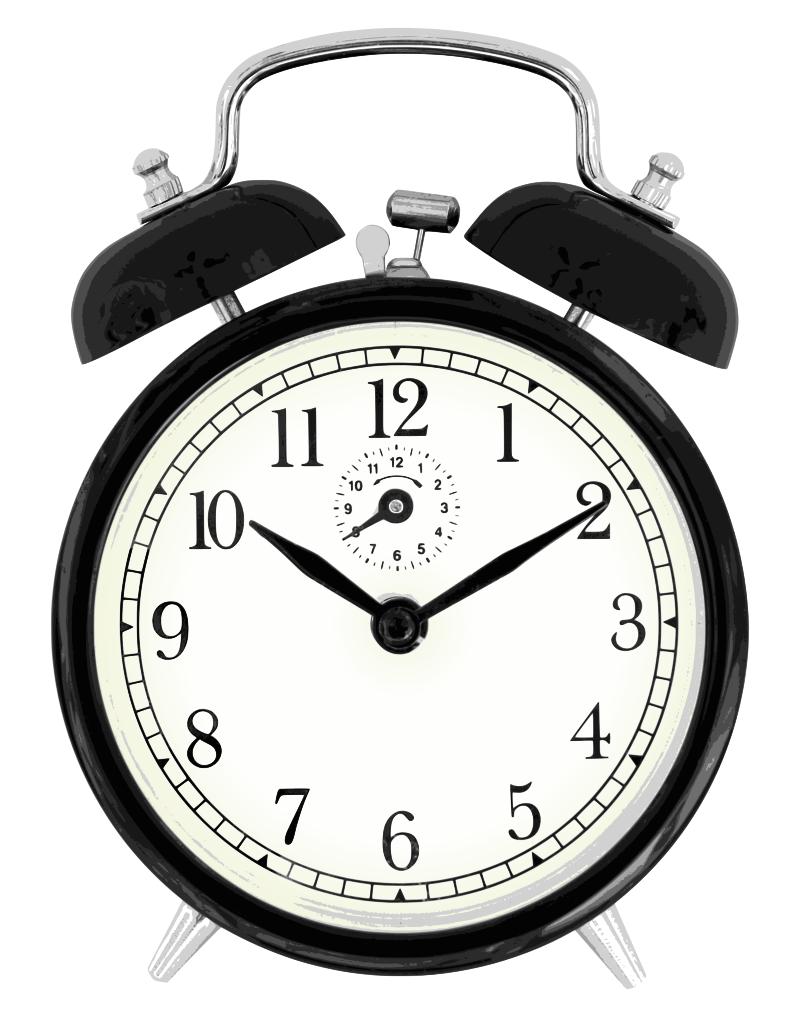
\includegraphics[width=6cm]{img/clock.png}}

%Make the Header
\makeatletter
\let\runauthor\@author
\let\runtitle\@title
\makeatother
\rhead{\runauthor}
\chead{\runtitle}
\lhead{\begin{picture}(0,0) \put(0,0){
\includegraphics[scale=0.5]{img/bfh.png}} \end{picture}}



\begin{document}

\thispagestyle{empty}
\maketitle
\tableofcontents

\pagestyle{fancy}


\begin{abstract}
\end{abstract}
\section{Zweck des Dokument}
TODO this is new text
%makes sure the whole glossary gets printed even when acronyms are not defined

\section{Kurzbeschreibung}
Das Ziel des Projektes ist einen Ersatz zum Programm kAlarm zu entwickeln.
Das Program kAlarm erlaubt es den User Benutzerdefinierte Erinnerungen zu erstellen. Mittels Pop-Up Windows wird der User dann zur gegebenen Zeit daran erinnert.
Im gegensatz zu kAlarm soll das zu erstellende Produkt Platformübergreifend verfügbar sein. Wie kAlarm soll dieses Produkt unter einer Open Source Lizenz entwickelt werden.
\section{Projektziele}
Unser Auftraggeber ist kein Unternehmen. Es werden somit auch keine Ziele innerhalb einer Unternehmens verfolgt.
Ziele welche ein Benuzer unsere Aplikaiton verfolgen könnte wären Beispielsweise:
\begin{itemize}
 \item Wiederkehrende Events nicht zu vergessen.
 \item An den Wäschetag erinnert weden.
 \item Die Wäsche rechtzeitig aus de Wäscheküche holen.
\item Den Kuchen nicht im Backofen verbrennen lassen.
 \item Der Sekretärin zum Geburtstag Blumen schicken.

\end{itemize}

\section{Stakeholders}
\begin{itemize}
\item{Auftragsgeber: Prof. Claude Furrer}
\item{Auftragsnehmer: Jonathan Hyams, Pascal Schmalz}
\item{Benutzer: FOSS Communitiy}
\end{itemize}
\section {Systemabgrenzung}
\subsection{Geschäftsprozesse}
Es existieren keine vor\- oder nachgelagerten Prozesse. Unsere Lösung lässt sich in beliebige viele Prozesse integrieren.
\subsection{Systeme}
Unser System wirkt mit Datebanken zusammen. Es baut auf Betriebsystemskomponenten auf. Namentlich Cronjob /Schtasks.
%TODO uml einbinden
\begin{landscape}
\begin{figure}
  \centering
    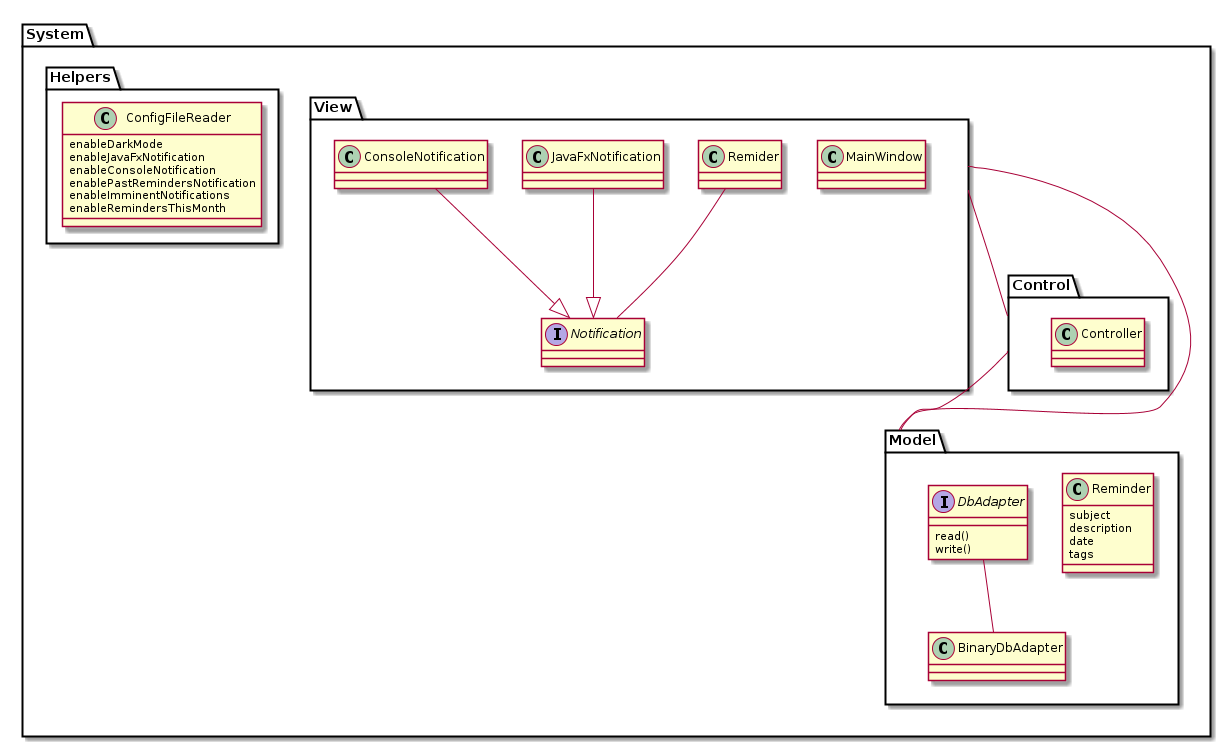
\includegraphics[width=1\textwidth]{../uml/uebersicht.png}
  \caption{Systemübersicht und Abgrenzung}
  \label{fig:overview}
\end{figure}
\end{landscape}
Die Systemübersicht und Abgrenzung Abb.~\ref{fig:overview} Seite~\pageref{fig:overview} bedient sich der UML Notation, ohne die UML Spezifikationvollständig einzuhalten.
\pageref{fig:overview}






Je nach gewünschter Notification Möglichkeiten kann mit E-Mails, SMS und Systemnotifications gearbeitet werden. Dies Bedingt, dass entsprechende Services / Server eingerichtet und über eine definierte Schnittstelle erreichbar sind.
\subsection{Randbedingungen}
Die Entwicklung soll mittels Java und JavaFX erfolgen.
Das Programm soll Betriebssystem und Datenbank agnostisch sein. Das Projekt muss unter einer Opensource Lizenz veröffentlicht werden.
Die Dokumentation muss in \LaTeX erstellt werden.


\subsection{Prozessumfeld}
\subsection{Systemumfeld}
\subsection{Randbedingungen}
\section{Anforderungen}
\subsection{Basisfaktoren}
\begin{itemize}

\item Die Schnittstelle zwischen dem Programmcode und der Datenbank soll so gestaltet sein, dass mit einem minimalen Aufwand eine beliebige gängige Datenabank genutzt werden kann.

\item
Die Schnittstelle zwischen dem Programmcode und der Datenbank soll so gestaltet sein, dass mit einem minimalen Aufwand eine beliebige Standard Datenbank genutzt werden kann.

\item
Die Bereitstellung eines JPA Drivers der Datenbank ist dabei nicht mehr im Scope des Projektes, sondern wird von den Datenbankherstellern oder von dritten vorgenommen.

\item
Das System muss dem Benutzer die Möglichkeit bieten, in dem GUI ein Einzelevent zu erfassen.
Das System sollte dem Benutzer die Möglichkeit bieten, über das GUI ein Einzelevent zu erfassen.

\item
Das System muss dem Benutzer die Möglichkeit bieten, in dem GUI wiederkehrende Events zu erfassen.
Das System sollte dem Benutzer die Möglichkeit bieten, über das CLI wiederkehrende Events zu erfassen.

\item
Das System kann anderen Programmen über eine API ermöglichen, Einzelevents zu erfassen.
Das System kann anderen Programmen über eine API ermöglichen, wiederkehrende Events zu erfassen.

\item
Das löschen und anpassen von Events soll wie oben beschrieben, ebenfalls möglich sein.

\item
Das System muss den Benutzer mittels einer Notification rechtzeitig auf ein Event hinweisen.

\item
Das Programm muss beim Programmstart seine Konfiguration mittels eines Configsfiles vorunehmen.

\item
Das Programm kann dem Benutzer die Möglichkeit bieten, die Konfiguration über die GUI vorzunehmen und im Configfile zu speichern.


\end{itemize}

\subsection{Leistungsfaktoren}
\begin{itemize}
\item
Der Benutzer soll neue Kategorien hinzufügen, anpassen und löschen können.
\item
Events sollen durch den Benutzer in Kategorien eingeteilt werden können.
\item
Der Benutzer soll Events nach Kategorien gruppieren und filtern können.
\item
Das Programm soll vorkonfigurierte Dienste vorausgesetzt, in der Lage sein Notifications als SMS und Emails zu versenden.
\item
Das Programm soll vorkonfigurierte Dienste vorausgesetzt, in der Lage sein anstelle einer Notification ein Script laufen zu lassen.
\item
Die GUI soll Benutzerzentriert und Ergonomisch sein (Wie kann man dies sinvoll als Anforderung formulieren?)
\end{itemize}

\subsection{Begeisterungsfaktoren}


\begin{itemize}
\item
Das Programm soll vorkonfigurierte Dienste vorausgesetzt, in der Lage sein anstelle einer Notification  ein IFTT Event auszulösen.

\item
Das Programm soll zusätzlich zu den gängigen Computer Betriebssystem auch auf Android lauffähig sein.

\item
Events sollen zwischen allen registrieren Geräten eines Registrierten Benutzers synchronisiert werden.Dazu muss der Benutzer in der Lage sein sich und seine Geräte,welche das Programm installiert haben, zu Registrieren.

\item
Das Programm soll auf den Betriebssystemen, welche eine Notificationinfrastruktur bereitstellen  in der Lage sein die Notifications über diese Notificationinfrastruktur vorzunehmen.(BSP KDE)

\item
Das Programm soll sich vom Loock and Feel in die jeweilige Desktop Environment anpassen.

\end{itemize}






 %IFTTT
\subsection{Quellen und Vorgehen}
Unsere wichtigste Quelle ist unser Auftraggeber Prof. Furrer. Um die Fragen, welche bei der Erstellung der Anforderungen aufgetaucht sind zu klären, werden wir uns mit ihm treffen.
Besondere folgende Fragen gilt es abzuklären:

\begin{itemize}
\item Entspricht die bisherige Ausarbeitung der Vorstellung des Auftraggebers.
\item vollständigkei der Anforderungen.
\item Kategoriserung der Anforderungen.
\item Priorisierung der Anforderungen.
\item Was soll mit der Eventkategorisierung erreicht werden, welche wieteren Anforderungen ergeben sich daraus.
\item Abgrenzung des Programmes gegenüber eines Kalenders und gegenüber des Cronjobs.
\end{itemize}
Da unser Auftraggeber als Professor der Informatik,
Als weitere Diskusionsgrundlage sind wir daran neben diesem Dokument einen Prototyp des GUI zu erstellen.


Die Angegebenen Informationen,insbesonder die abzuklärenden Punkte, sind dementsprechend lediglich eine Work in Progress.


Als weitere Qullen können wir die Dokumentation und Code Basis von kAlarm nutzen.
Da wir selber der potentiellen Nutzergrupp des Programmes angehören, könneten wir auch uns selber als Quelle nutzen, als Entwickler hat man jedoch oft einen anderen Blickwinkel als ein normaler Benutzer.


Im sinne einer Agilen Entwicklung wollen wir möglichst rasch präsentierbare Artefakte generieren, damit der Auftraggeber frühstmöglich Einfluss nehmen kann und Fehlentwicklungen vermieden werden. Treffen werden bei bei bedarf mit dem Auftraggeber ausgemacht.


\subsection{Technische Anforderungen}
\subsection{Qualitätsanforderungen}
\section{Glossar}
\listoffigures
\listoftables
%TODO bibography

\glsaddall
\printglossary
\section{Anhang}

\subsection{Abstimmung der Anforderungen}
\subsection{Definition of Ready - Checklist}
\section{Versionskontrolle}
Manuelle Version: 0.0.2
\\

\noindent
Automatische Versionierung:
%\immediate\write18{../script/printGitVersionNumber.sh}
%\input{automaticGitVersionNumber}
%git rev-list --count --first-parent HEAD
%9	Literaturverzeichnis	4

\immediate\write18{../script/versionInfo.sh}
Fetching version information failed. Please enable shell-escape in your \LaTeX \~  compiler.

\immediate\write18{../script/cleanup.sh}
%\immediate\write18{../script/clean.sh}







\end{document}
